\documentclass[aspectratio=169]{beamer}
\usepackage[utf8]{inputenc}
\usepackage[T1]{fontenc}
\usepackage[brazil]{babel}
\usepackage{ragged2e}
\usepackage{booktabs}
\usepackage{verbatim}
\usetheme{AnnArbor}
\usecolortheme{orchid}
\usefonttheme[onlymath]{serif}

\AtBeginSection[]{
  \begin{frame}
  \vfill
  \centering
  \begin{beamercolorbox}[sep=8pt,center,shadow=true,rounded=true]{title}
    \usebeamerfont{title}\insertsectionhead\par%
  \end{beamercolorbox}
  \vfill
  \end{frame}
}

\title[\sc{Introdução à Orientação a Objetos}]{Introdução à Orientação a Objetos}
\author[Roland Teodorowitsch]{Roland Teodorowitsch}
%\institute[LP2 - EC - PUCRS]{Laboratório de Programação II - Curso de Engenharia de Computação - PUCRS}
\institute[POO - EC - PUCRS]{Programação Orientada a Objetos - ECo - Curso de Engenharia de Computação - PUCRS}
\date{1 de setembro de 2021}

\begin{document}
\justifying

%-------------------------------------------------------
\begin{frame}
	\titlepage
\end{frame}

%=======================================================
\section{Conceitos}

%-------------------------------------------------------
\begin{frame}\frametitle{Paradigma Programação}
\begin{itemize}
	\item É uma forma de se classificar as linguagens de programação a partir de suas funcionalidades
	\item É um padrão conceitual que orienta soluções de projeto e implementação
	\item Fornece e determina a visão que o programador possui sobre a estruturação e execução de seus programas
	\item Paradigmas explicam como os elementos que compõem um programa são organizados e como interagem entre si
	\item Exemplos: procedural, funcional, orientado a objetos
	\item Uma linguagem pode suportar mais de um paradigma
	\item Um programa pode NÃO aproveitar as funcionalidades de um paradigma
\end{itemize}
\end{frame}

%-------------------------------------------------------
\begin{frame}\frametitle{Programação Orientada a Objetos}
\begin{itemize}
	\item É um modelo de análise, projeto e programação de \emph{software} baseado na composição e interação entre unidades chamadas de \textbf{objetos}
	\item É um estilo de programação que se baseia na modelagem de \textbf{objetos} do mundo real
\end{itemize}
\end{frame}

%-------------------------------------------------------
\begin{frame}\frametitle{Objetos}
\begin{itemize}
	\item São entidades que pode ser facilmente reconhecidas
	\item São abstrações de objetos do mundo real
	\item Um objeto é uma estrutura composta de:
	\begin{itemize}
		\item \textbf{atributos}: características ou dados
		\item \textbf{comportamentos}: operações, interface ou métodos
	\end{itemize}
	\item Exemplos:
	\begin{itemize}
		\item caneta
		\begin{itemize}
			\item características: cor da tinta, quantidade de tinta, etc.
			\item comportamento: escrever, recarregar, etc.
		\end{itemize}
		\item lâmpada
		\begin{itemize}
			\item características: ligada (sim/não), potência, voltagem, etc.
			\item comportamento: ligar, desligar, queimar, etc.
		\end{itemize}
	\end{itemize}
\end{itemize}
\end{frame}

%-------------------------------------------------------
\begin{frame}\frametitle{Programa Orientado a Objetos}
\begin{itemize}
	\item É estruturado como um conjunto de objetos que interagem entre si
	\item Cada objeto tem um papel a cumprir
	\item Cada objeto oferece um serviço ou realiza uma ação que é usada por outros membros do conjunto
	\item Exemplo: um computador e seus diversos componentes (teclado, mouse, vídeo, UCP, etc.)
\end{itemize}
\end{frame}

%-------------------------------------------------------
\begin{frame}\frametitle{Abordagem OO}
\begin{itemize}
	\item Princípios da abordagem OO
	\begin{itemize}
		\item \textbf{Abstração}: representação de um objeto do mundo real, ``abstraindo-se'' os detalhes desnecessários, de forma que o objeto possa ser utilizado sem se preocupar com como ele foi implementado
		\item \textbf{Encapsulamento}: detalhes da implementação ficam escondidos e a manipulação dos dados acontede através de uma interface pública
		\item \textbf{Modularidade}: vários componentes que interagem
	\end{itemize}
	\item Abstração, Encapsulamento, Herança e Polimorfismo são considerados os 4 pilares da POO
\end{itemize}
\end{frame}

%-------------------------------------------------------
\begin{frame}\frametitle{Encapsulamento}
\begin{itemize}
	\item É um dos conceitos básicos da OO
	\item A ideia é que cada objeto seja uma ``caixa preta'':
	\begin{itemize}
		\item Não é necessário saber os detalhes de seu funcionamento interno
		\item Basta saber como utilizá-lo
	\end{itemize}
	\item Encapsular é esconder como as coisas funcionam (\emph{data hiding}) por trás de uma interface externa (pública)
	\item Exemplo: termostado
	\begin{itemize}
		\item Aciona um dispositivo a partir de determinada temperatura
		\item Como ele é implementado internamente?
		\item Como pode ser usado?
	\end{itemize}
\end{itemize}
\end{frame}

%-------------------------------------------------------
\begin{frame}\frametitle{Encapsulamento}
\begin{itemize}
	\item Um objeto é formado por:
	\begin{itemize}
		\item Dados (Atributos):
		\begin{itemize}
			\item São \textbf{privado}
			\item Acesso aos dados deve ser feito através da chamada de um método
		\end{itemize}
		\item Operações (Métodos):
		\begin{itemize}
			\item São \textbf{públicos}
			\item Interface pública declara as operações permitidas
		\end{itemize}
	\end{itemize}
\end{itemize}
\end{frame}

%-------------------------------------------------------
\begin{frame}\frametitle{Benefícios do Encapsulamento}
\begin{itemize}
	\item A implementação interna de um objeto pode mudar e o resto do sistema não é afetado (desde que a interface de acesso não mude)
	\item Maior segurança ao proteger os atributos de um objeto de alterações indevidas por outros objetos
	\item Maior independência entre os objetos, pois eles só precisam conhecer a interface externa definida
\end{itemize}
\end{frame}

%-------------------------------------------------------
\begin{frame}\frametitle{Abstração}
\begin{itemize}
	\item Quando modelando um objeto, identificamos \textbf{somente} as operações e atributos que são essenciais
	\item Exemplo: caneta
	\begin{itemize}
		\item Atributos não modelados: fabricante, etc.
		\item Operações não modeladas: apontar, etc.
	\end{itemize}
\end{itemize}
\end{frame}

%-------------------------------------------------------
\begin{frame}\frametitle{Classes}
\begin{itemize}
	\item Uma classe é uma ``forma'' para produzir objetos
	\item Determina um conjunto de objetos com:
	\begin{itemize}
		\item Propriedades semelhantes
		\item Comportamentos semelhantes
		\item Relacionamentos comuns com outros objetos
	\end{itemize}
\end{itemize}
\end{frame}

%-------------------------------------------------------
\begin{frame}\frametitle{Instâncias}
\begin{itemize}
	\item \textbf{Instanciar} objetos significa gerar novos exemplares a partir de uma descrição abstrata de um objeto genérico (ou seja, de uma classe)
	\begin{itemize}
		\item Objetos são instâncias de uma classe
	\end{itemize}
\end{itemize}
\begin{figure}[h]
	\centering
	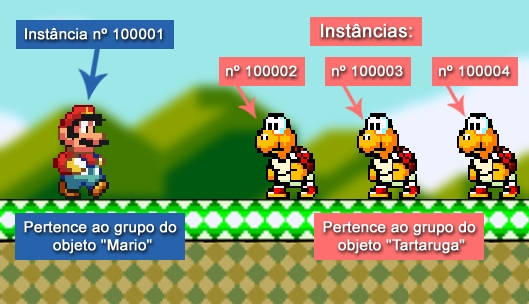
\includegraphics[height=0.5\paperheight]{imagens/instancias.jpg}
\end{figure}
\end{frame}

%-------------------------------------------------------
\begin{frame}\frametitle{Classes x Instâncias x Objetos}
\begin{itemize}
	\item Objetos são gerados a partir de classes
	\item Uma classe define as propriedades e o comportamento dos objetos gerados por ela
	\item Todo objeto é uma instância de uma classe
\end{itemize}
\end{frame}

%-------------------------------------------------------
\begin{frame}\frametitle{Classes x Instâncias x Objetos}
\begin{figure}[h]
	\centering
	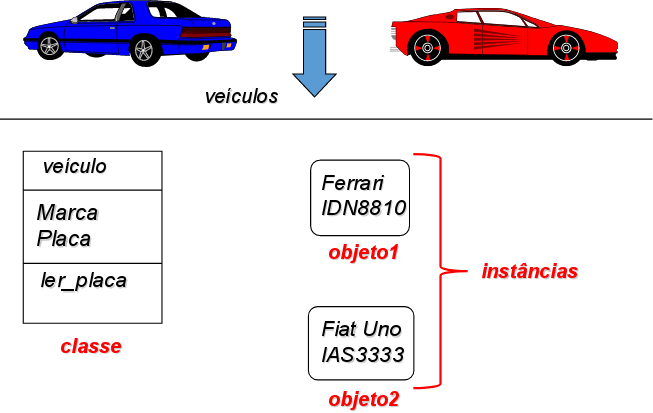
\includegraphics[height=0.7\paperheight]{imagens/carros.png}
\end{figure}
\end{frame}

%-------------------------------------------------------
\begin{frame}\frametitle{Exemplo em C++}
\begin{figure}[h]
	\centering
	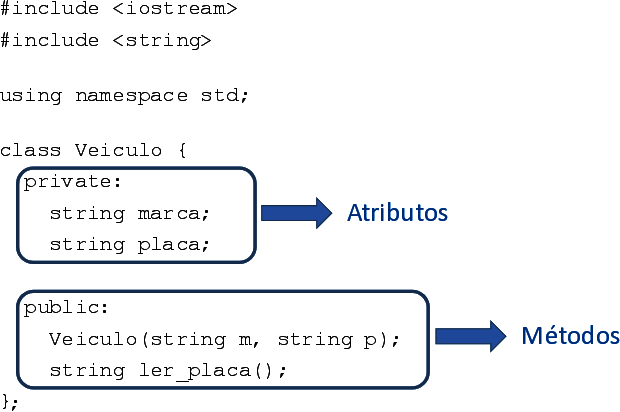
\includegraphics[height=0.7\paperheight]{imagens/exemplo_c++.png}
\end{figure}
\end{frame}

%-------------------------------------------------------
\begin{frame}\frametitle{Objetivo da POO}
\begin{itemize}
	\item Gerar programas que sejam:
	\begin{itemize}
		\item Legíveis e de fácil compreensão
		\item Reutilizáveis
		\item De fácil manutenção
		\item Obtidos de forma produtiva
	\end{itemize}
\end{itemize}
\end{frame}

%-------------------------------------------------------
\begin{frame}\frametitle{Resumo: Conceitos de OO}
\begin{itemize}
	\item Objeto
	\begin{itemize}
		\item Unidade básica de orientação a objetos
		\item É uma entidade que tem atributos, comportamento e identidade
		\item É um membro de uma classe e os atributos e o comportamento (métodos) de um objeto são definidos pela classe
	\end{itemize}
	\item Classe
	\begin{itemize}
		\item É uma descrição de um conjunto de objetos
		\item Este conjunto de objetos compartilha atributos e comportamento em comum
		\item Uma definição de classe descreve todos os atributos dos objetos membros da classe, bem como os métodos que implementam o comportamento destes membros
	\end{itemize}
\end{itemize}
\end{frame}

%-------------------------------------------------------
\begin{frame}\frametitle{Resumo: Conceitos de OO}
\begin{itemize}
	\item Orientação a objetos
	\begin{itemize}
		\item Um método de desenvolvimento de \emph{software} que usa abstração com objetos, classes encapsuladas e comunicação por mensagens, hierarquia de classes e polimorfismo
	\end{itemize}
	\item Abstração
	\begin{itemize}
		\item Um modelo de um conceito ou objeto do mundo real
	\end{itemize}
	\item Encapsulamento
	\begin{itemize}
		\item Processo de esconder os detalhes internos de um objeto do mundo externo
	\end{itemize}
	\item Atributo
	\begin{itemize}
		\item Usado para armazenar o estado de um objeto
		\item Pode ser simples como uma variável escalar (\texttt{int}, \texttt{char}, \texttt{double} ou \texttt{bool}) ou pode ser uma estrutura complexa tal como outro objeto
	\end{itemize}
\end{itemize}
\end{frame}

%-------------------------------------------------------
\begin{frame}\frametitle{Resumo: Conceitos de OO}
\begin{itemize}
	\item Comportamento
	\begin{itemize}
		\item Atividade de um objeto que é vista do ponto de vista do mundo externo
		\item Inclui como um objeto responde a mensagens alterando seu estado interno ou retornando informação sobre seu estado interno
	\end{itemize}
	\item Método
	\begin{itemize}
		\item Uma operação ou serviço executado sobre o objeto, declarado como parte da estrutura da classe
		\item Métodos são usados para implementar o comportamento do objeto
	\end{itemize}
	\item Estado
	\begin{itemize}
		\item Reflete os valores correntes de todos os atributos de um objeto e são o resultado do comportamento do objeto ao longo do tempo
	\end{itemize}
\end{itemize}
\end{frame}

%=======================================================
\section{Exemplo}

%-------------------------------------------------------
\begin{frame}\frametitle{Projetando Objetos}
De uma forma simples, o \textbf{projeto orientado a objetos} de um sistema pode ser dividido em três etapas:
\begin{enumerate}
	\item Identificar as abstrações/entidades envolvidas no problema
	\item Identificar os serviços que cada uma destas entidades deve ser capaz de fornecer
	\item Identificar os relacionamentos entre essas entidades
\end{enumerate}
\end{frame}

%-------------------------------------------------------
\begin{frame}\frametitle{Exemplo}
\begin{itemize}
	\item Deseja-se criar um sistema de cadastro de produtos que são vendidos em um supermercado. Cada produto possui uma descrição e um valor de venda. O sistema permite a emissão de relatórios dos produtos disponíveis. Também, é permitido ao gerente aplicar reajustes de preços sobre o produto que desejar.
\end{itemize}
\end{frame}

%-------------------------------------------------------
\begin{frame}\frametitle{Exemplo}
\begin{figure}[h]
	\centering
	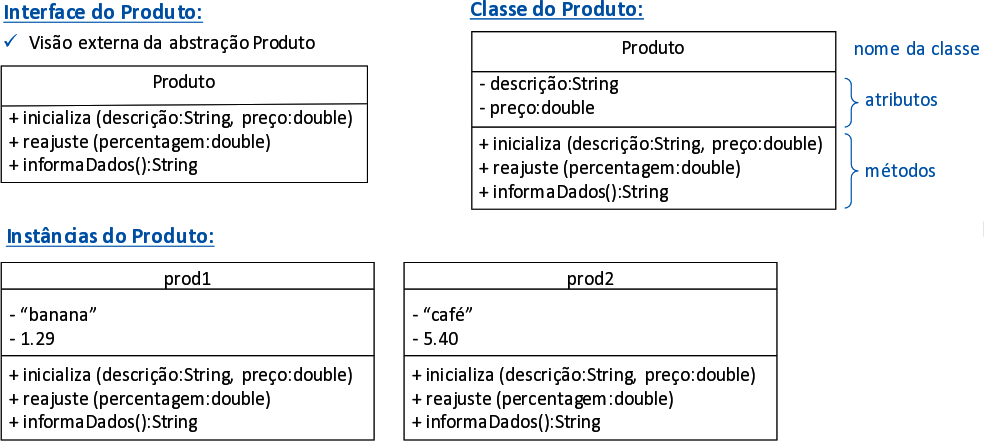
\includegraphics[height=0.7\paperheight]{imagens/modelagem.png}
\end{figure}
\end{frame}

%=======================================================
\section{Créditos}

%-------------------------------------------------------
\begin{frame}\frametitle{Créditos}
\begin{itemize}
	\item Estas lâminas contêm trechos de materiais disponibilizados pelos professores Rafael Garibotti e Edson Moreno.
\end{itemize}
\end{frame}

%-------------------------------------------------------
\end{document}

